\section{Généralités sur les images numériques}
    \subsection{Qu'est-ce qu'une image numérique ?}
    Une image numérique est toute image (dessin, icône, photographie …) acquise, créée, traitée ou stockée sous forme binaire (suite de 0 et de 1) :
    \begin{itemize}
        \item[•]\textbf{Acquise} par des dispositifs comme les scanners, les appareils photo ou caméscopes numériques, les cartes d’acquisition vidéo (qui numérisent directement une source comme la télévision).
        \item[•]\textbf{Créée} directement par des programmes informatiques, via la souris, les tablettes graphiques ou par la modélisation 3D (ce que l’on appelle par abus de langage les « images de synthèse »).
        \item[•]\textbf{Traitée} grâce à des outils informatiques. Il est facile de la modifier en taille, en couleur, d’ajouter ou supprimer des éléments, d’appliquer des filtres variés, etc.
        \item[•]\textbf{Stockée} sur un support informatique (disquette, disque dur, CD-ROM(Compact Disk Read Only Memory), …) \cite{wikiImage}
    \end{itemize}
    \subsection{Représentation de l'image}
    Selon la manière dont les images sont représentées pour être visualisées sur les écrans des ordinateurs, on distingue deux grandes classes d’images numériques:

    \begin{itemize}
        \item[•]\textbf{Les images matricielles}: Encore appelées images bitmap, elles sont représentées à travers des matrices de points à plusieurs dimensions. Dans le cas de deux dimensions spatiales (largeur, hauteur), on parle d’\textbf{images 2D} et les points sont appelés \textbf{pixels (Picture Element)}. C’est le type le plus répandu. Si une image 2D possède en plus un composant temporel \textbf{(image 2D + t)}, on parle dans ce cas d’\textbf{animation}. Si par contre l’image possède trois dimensions spatiales (largeur, hauteur, profondeur), on parle d’\textbf{image 3D} ou volume et les points sont appelés \textbf{voxels (Volume Element)}.
        \item[•]\textbf{Les images vectorielles}: Les données d'une image vectorielle sont représentées par des formes géométriques (cercle, rectangle, ...) qui sont décrites mathématiquement. Elles possèdent l’avantage contrairement aux images vectorielles d’occuper moins d’espace mémoire et la flexibilité dans le redimensionnement sans perte d’informations.
    \end{itemize}
    \begin{figure}
        \centering
        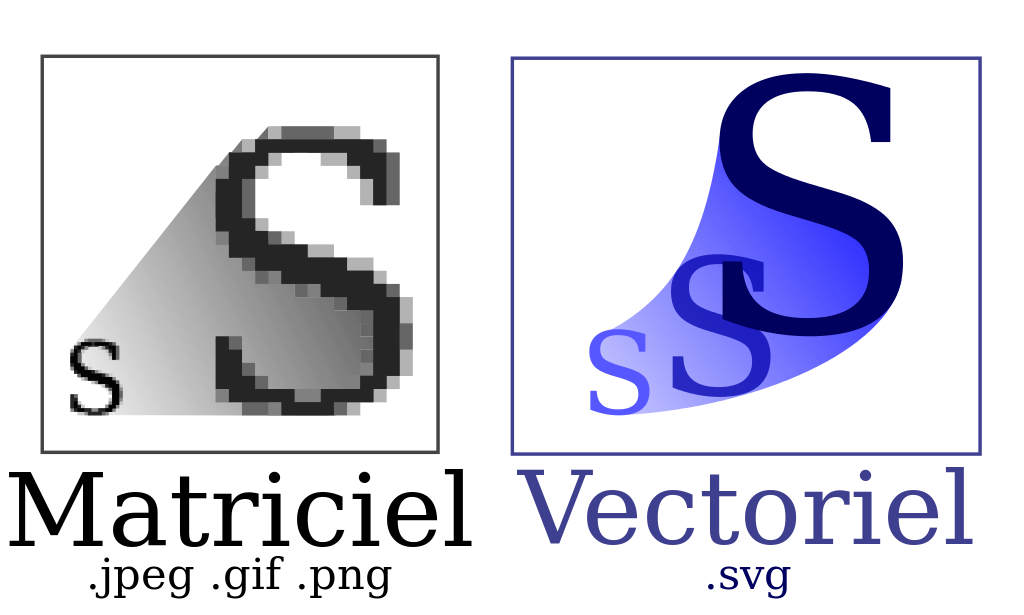
\includegraphics[scale=0.3]{matricielleVSvectorielle}
        \captionsource{Différence entre image matricielle et image vectorielle}{\href{https://www.imedias.pro/cours-en-ligne/graphisme-design/definition-resolution-taille-image/les-images-vectorielles-matricielles/}{Site Cours en ligne}}
    \end{figure}
    Dans la famille des images matricielles, on distingue trois types d’images:
    \begin{itemize}
        \item[•]\textbf{Les images binaires}: Elles sont uniquement en noir et blanc. La matrice de représentation contient uniquement des 0 et 1.
        \item[•]\textbf{Les images en niveaux de gris}: La matrice de représentation contient des valeurs entières entre 0 et 255 qui correspondent au niveau d’intensité lumineuse.
        \item[•]\textbf{Les images de couleur}: Elles sont régulièrement obtenues par une synthèse additive des trois couleurs fondamentales :rouge, vert, bleu (RVB ou RGB en anglais). La matrice de représentation est constituée dans ce cas de trois matrices: pour chaque couleur, une matrice dont chaque cellule donne l’intensité lumineuse de la couleur correspondante.
    \end{itemize}
    \begin{figure}
        \begin{subfigure}{0.3\textwidth}
            \centering
            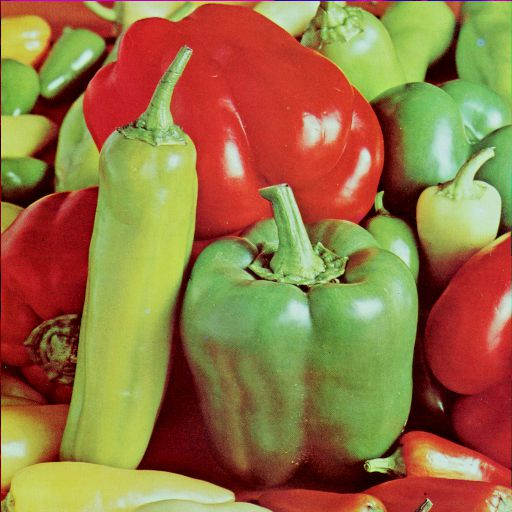
\includegraphics[width=\textwidth]{food}
            \caption{Image de couleur}
        \end{subfigure}
        \hfill
        \begin{subfigure}{0.3\textwidth}
            \centering
            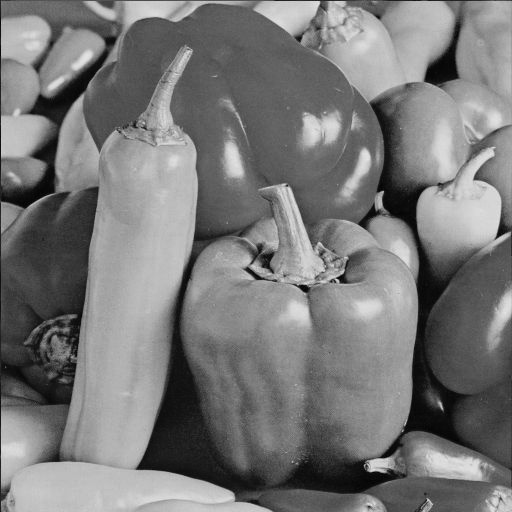
\includegraphics[width=\textwidth]{food_gray}
            \caption{Image en niveau de gris}
        \end{subfigure}
        \hfill
        \begin{subfigure}{0.3\textwidth}
            \centering
            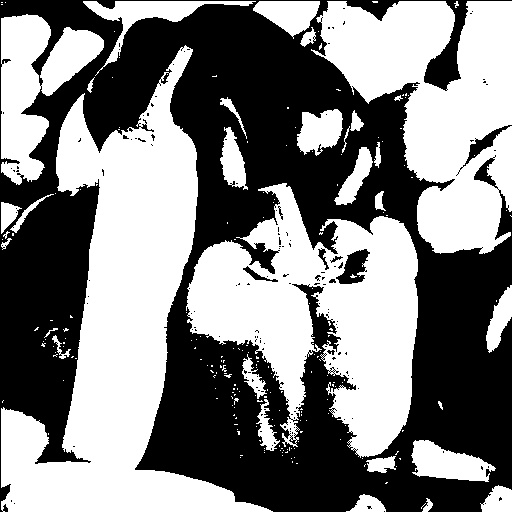
\includegraphics[width=\textwidth]{food_binary}
            \caption{Image binaire}
        \end{subfigure}
        \caption{Exemples de types d'images matricielles}
    \end{figure}
	Dans le cadre de notre projet, nous travaillons exclusivement avec les images matricielles 2D. Donc pour la suite, lorsqu’on parle d’image, il s'agit d’une image matricielle 2D sauf s’il est mentionné le contraire. 
    \subsection{Caractéristiques d'une image numérique}
    Une image a trois caractéristiques principales:
    \begin{itemize}
        \item[•]\textbf{Les dimensions}: Elles représentent la largeur et la hauteur de l’image généralement exprimées en pixels.
        \item[•]\textbf{La définition}: C’est le nombre de pixels constituant une image. Elle est obtenue en multipliant le nombre de pixels sur la largeur par le nombre de pixels sur la hauteur.
        \item[•]\textbf{La résolution}: C’est le nombre de pixels que l’on retrouve sur une unité de longueur. Elle s’exprime généralement en ppp (point par pouce) ou encore en anglais dpi (dot per inch).  Plus la résolution est importante, plus les points sont petits et nombreux, plus l’image est fine.
    \end{itemize}

    \subsection{Formats des images numériques}
    Le format d’une image est la représentation informatique de cette image. Il donne les informations nécessaires sur la manière dont l’image a été codée et éventuellement des moyens de la décoder et de la manipuler. Il existe plusieurs formats qui plus ou moins adaptés pour certains cas d’utilisation:

    \begin{itemize}
        \item[•]\textbf{Format \acrfull{gif}}: Ce format permet la transparence et les images animées plusieurs images séquentielles à l’intérieur du même fichier. Il est utilisé pour des logos, des icônes, des boutons et autres éléments de pages web.Le format d’image GIF n’atteigne au maximum que 256 couleurs, il n’est donc pas du tout adapté aux photos et à l’impression.
        \item[•]\textbf{Format \acrfull{tiff}}: Un des formats le plus couramment utilisé pour stocker des images, des photographies.Il est couramment utilisé dans les environnements professionnels et pour l’impression commerciale. Il est considéré comme étant le format le plus fiable pour des impressions de haute qualité comme pour le textile, les tissus.
        \item[•]\textbf{Format \acrfull{jpg}}: C’est le format le plus adéquat pour administrer ses photos et les publier. Un des formats les plus utilisés sur le net (les navigateurs l’affichent correctement), et dans les mails. Les appareils photo numériques compacts prennent également les photos au format JPG.
        \item[•]\textbf{Format \acrfull{png}}: Un des formats le plus couramment utilisé. Créé pour remplacer le GIF il est très peu connu du grand public. Performant, il réunit presque tous les avantages du JPEG et du GIF et permet les fonds transparents. La compression proposée par ce format est perte d’une qualité 5 à 25 \% meilleure que la compression GIF. \cite{akacemMaster}
        \item[•]\textbf{Format \acrfull{svg}}: Contrairement aux précédents formats, SVG est un format d’images vectorielles. Il est conçu pour décrire un ensemble de graphiques vectoriels en utilisant XML. Cette conception permet aux images sous ce type de format d’être agrandies à l’infini sans impact sur la qualité. On utilise généralement ce format pour échanger des graphiques sur internet ou dans des logiciels de dessin assisté par ordinateur(DAO) pour représenter les objets.    
    \end{itemize}